\section{Preliminary Results}
\label{sec-results}

To explore the potential to transform our discarded Nexus~S~4G smartphones
into low-power sensors, the authors divided into two teams and engaged in a
lifetime programming competition. Each team was provided five discarded
Nexus~S~4G phones and given two weeks to write a program that recorded
battery and light levels every 15~minutes and transmitted them to a server
over a Wifi connection. The goal was to implement a sensing application that
would last as long as possible, while maintaining data delivery to the
server. A gap of over two hours in the data values as observed by the other
team rendered the node as dead, regardless of the amount of energy it had
reported, with the two hour delay chosen to represent the potential
requirements of a somewhat delay-tolerant application.

\begin{figure}[t]
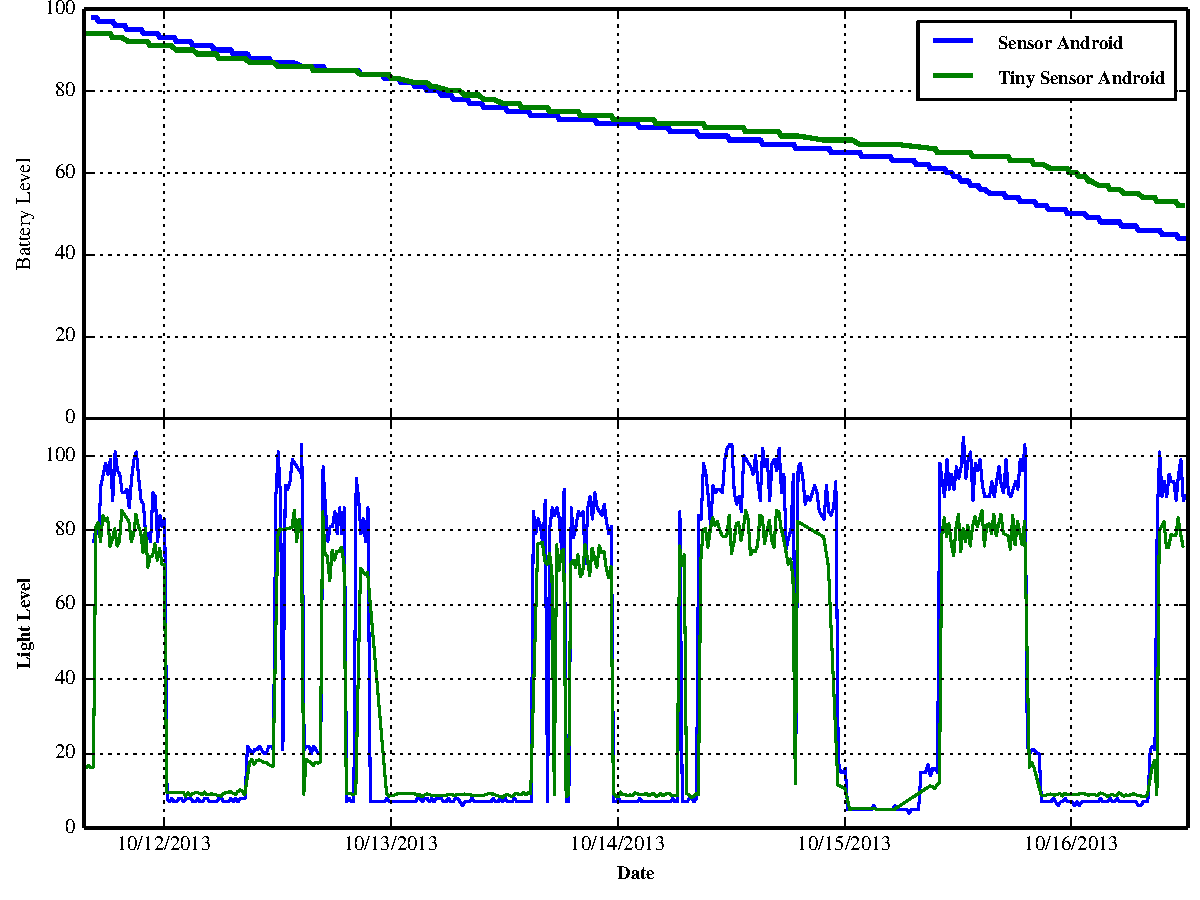
\includegraphics[width=\columnwidth]{./figures/comparison.pdf}

\caption{\small Lifetime results for two light sensing applications.
\textnormal{Both the Tiny Sensor Android (Section~\ref{subsec-tiny}) and
Sensor Android (Section~\ref{subsec-full}) approaches were projected to
achieve a lifetime of 8--9 days.}}

\label{fig-comparison}
\end{figure}


\XXXnote{Overall results.}

Broadly speaking the teams both explored two different options with important
implications for reuse in this context: starting with a stock AOSP platform
build and the familiar Android API, or using a super-minimal Tiny Android
build that discards most of the platform components. We refer to the first
approach as ``Sensor Android'' and the second as ``Tiny Sensor Android''.
From a programming perspective, we were hopeful that we could preserve the
familiar Android environment that many programmers today are learning. But
from an energy management persective, we were worried that the platform
contained features designed around short lifetimes that would prove
unhelpful. We describe both approaches in more detail below.

\subsection{Tiny Sensor Android}
\label{subsec-tiny}

Tiny Android is a development option enabling a stripped-down build intended
for testing new devices, and was not suitable for our application without
modifications. Wifi drivers had be added to the build process, and these
created several other dependencies. Our Tiny Sensor Android build added
\XXXnote{GWA : Guru TODO} packages to the \XXXnote{GWA : Guru TODO} normally
used by Tiny Android.

\XXXnote{GWA : Guru TODO : One or two paragraphs about the implementation.}

Figure~\ref{fig-tinyandroid} shows current output for one sense-and-send
cycle of our sensing application on Tiny Sensor Android. While the sensing
and transmission complete quickly, allowing the phone to rapidly return to
idle, there was an extra 8~mA of current during the idle state which we have
yet to explain. We believe it may be caused by \XXXnote{GWA : Guru TODO}.

\subsection{Sensor Android}
\label{subsec-full}

\XXXnote{GWA: Anand TODO} 

\subsection{Comparison}
